\clearpage

\setcounter{chapter}{3}
\setcounter{section}{0}
% Add the chapter to table of contents
\addcontentsline{toc}{chapter}{\numberline{3}From Theory to Practice - Experimental Pathways}


% Set up page style for this chapter (assuming fancyhdr is loaded in preamble)
\pagestyle{fancy}
\fancyhf{} % Clear all header and footer fields
\fancyhead[L]{\footnotesize\textit{Ars Post Faber: Digital Fabrication Democratization Through Embodied Knowledge Preservation}}
\fancyfoot[C]{\thepage} % Page number in footer center
\renewcommand{\headrulewidth}{0pt}
\renewcommand{\footrulewidth}{0pt}


% Custom chapter title to match abstract formatting
\noindent
{\Large\textbf{Chapter 3: Developing Theory From Practice, Experimental Pathways}}
\vspace{0.3cm}
\hrule
\vspace{0.8cm}
\label{ch:experimental_pathways}

% Set no paragraph indentation
\setlength{\parindent}{0pt}
The theoretical framework developed in the previous chapters suggested that genuine democratization of digital fabrication requires preservation-based approaches that maintain adaptive authority rather than simply expanding access to predetermined tools. Yet this analysis raised questions about implementation: \textit{How might such preservation actually operate within existing technological contexts?} \textit{Could alternative "interfaces" bridge the gap between computational precision and embodied expression?} The following interventions sought to address these questions through practical experiments that tested the theoretical propositions in real-world making contexts.

\vspace{0.5cm}

This chapter will document different "interventions" that progressively refined approaches to preserving the embodied knowledge within digital workflows. Each experiment built upon insights from the previous, leading to the development of \textit{Ars Post Faber}, the open-source Grasshopper\footnote{Grasshopper is a visual programming language and environment that runs within the Rhinoceros 3D computer CAD software. Developed by David Rutten at Robert McNeel \& Associates, Grasshopper enables users to build generative algorithms through a node-based interface without requiring traditional programming knowledge, making it widely used in parametric design, digital fabrication, and computational design workflows.} plugin\footnote{A plugin (also called an add-on or extension) is a software component that adds specific functionality to an existing program. In the context of CAD and design software, plugins extend the applications capabilities by providing new tools, commands, or workflows. They are typically developed by third parties and can be installed and removed without modifying the main software, allowing users to customize their design environment for specific tasks or methodologies.} that embodies the research's theoretical conclusions.

\section{\textit{CR3ATED}: Reimagining CAD Interfaces for Artisan Expression}
\textit{"If craftsmanship's essence lies in the creative problem solving process, how can digital fabrication tools become active participants in it rather than automation devices?"}

\vspace{0.5cm}

\subsection{Exploring Alternative Interface Approaches}

Building upon insights from AI.RTISANSHIP, it was concluded that computational systems could successfully capture and analyze certain patterns of skilled movement, yet this technical capability highlighted a bigger challenge where the preserved data represented only "surface" manifestations of embodied knowledge rather than the adaptive reasoning processes. This raised a different question: \textit{Rather than attempting to extract embodied knowledge from practitioners, what if digital tools could be designed to better support and amplify the adaptive decision-making processes that characterize skilled practice?}

\vspace{0.5cm}

This inquiry led to the development of \textit{CR3ATED}, a web-based application designed to test alternative interface approaches within digital design and fabrication workflows. Where AI.RTISANSHIP looked to decode existing craft knowledge through computational analysis, \textit{CR3ATED} explored how interface design itself might preserve creative expression by exploring different human-software interactions.

\vspace{0.5cm}

The \textit{CR3ATED} experiment investigated whether alternative modes of human-software interaction could maintain the continuity between creative intention and material execution that conventional CAD workflows tend to fragment. The central hypothesis was that interface design actively constructs the kinds of creative relationships that become possible within digital fabrication workflows, suggesting that preserving craft agency might require different approaches to how makers engage with computational design tools.

\subsection{Craftinnova: Testing Alternative Interfaces}

The CR3ATED web application was developed specifically for the "Nuevos Métodos de Aprendizaje Artesano" workshop at CRAFTINNOVA\footnote{CRAFTINNOVA is Spain's national event combining artistic crafts and innovation, held annually in Valladolid. The event brings together creators, designers, manufacturers, technology experts, digital fabrication professionals, artists, entrepreneurs, and makers to explore the intersection of traditional craftsmanship with digital technologies.}, creating an opportunity to test these alternative interface approaches with practicing artisans in a real-world context. The workshop brought together traditional craftspeople with clay 3D printing technology, creating an ideal laboratory for investigating how interface design affects the preservation of creative expression.

\vspace{0.5cm}

Rather than using conventional CAD software, the webapp, implemented a touch-based sketching interface that allowed participants to create 3D models through direct manipulation on mobile devices. The application translated 2D sketches into revolution surfaces suitable for clay printing, maintaining the intuitive hand-to-head connection that characterizes crafts while engaging with the digital fabrication capabilities of the machine.

\vspace{0.5cm}

This approach acknowledged that conventional CAD systems fail to express the imperfection and responsiveness from the craft practice. By creating a workflow that began with tactile sketching and culminated with material engagement, the experiment explored how technology might contribute to craft preservation by becoming integrated into evolving creative practice rather than replacing traditional methods.

\subsection{Material Continuity and Digital Mediation}

An important aspect of the workflow developed involved preserving material continuity between digital design and physical fabrication. The clay printer, despite its digital control system, interacts with clay according to the same physical principles that govern hand techniques, unlike the normally used polymers in additive manufacturing that cannot be hand-treated. Clay maintains its material properties regardless of whether it is shaped by hand or extruded through a mechanical nozzle, maintaining material coherence across the digital/physical boundary.

\vspace{0.5cm}

This materiality creates productive constraints rather than arbitrary limitations. Workshop participants encountered the clay printer's capabilities and limitations as a new set of material conditions to navigate, drawing on their traditional knowledge while developing new skills specific to the printer. Unlike conventional CAD/CAM workflows that abstract away material properties through geometric representation, the \textit{CR3ATED} approach maintained material feedback throughout the process.

\vspace{0.5cm}

The touch interface proved to be important for preserving this material relationship. Whereas CAD requires learning abstract geometric manipulation techniques, sketching with the finger or a stylus maintains the tactile connection between hand movement and form development. Participants of the workshop were able to leverage their existing skills while engaging with digital fabrication, rather than having to master entirely new representational systems.

\subsection{Expanding vs. Replacing Practice}

The workshop generated diverse responses from the participants, showing different ways that digital tools might relate to traditional practice. For most, the clay printing process represented a new exploration rather than a shift in their approach. These artisans engaged with the technology as they might with any new tool or technique, integrating it within their existing practice. However, other participants experienced the workshop as an expansion of their literacy in both digital and material domains. For these makers, the interface exploration enabled forms of creative expression and production that would have been difficult (or impossible) to achieve through either traditional hand-building or conventional CAD approaches.

\vspace{0.5cm}

At it's core, the workshop attempted to challenge the binary thinking that has historically characterized discussions of technology and craft. Rather than facing off hand-building versus digital printing as competing methodologies, the comparison between techniques became "an exploration of their complementary strengths" rather than a contest between "superior" and "inferior" approaches. Aligning with Gershenfeld's vision of personal fabrication enabling the convergence of industrial production with personal expression, "which would merge with digital design, to bring common sense and sensibility to the creation and application of advanced technologies" (Gershenfeld, 2007). The clay printer became not merely a tool but a participant in creative dialogue, presenting its own challenges and possibilities while requiring new skills that built upon traditional knowledge.

\vspace{0.5cm}

\subsection{Success and Limitations of the Experiment}

Despite the "success" in exploring a new way of interaction and preserving material relationships, the intervention highlighted certain limitations that pointed towards the need for more sophisticated future experiments. While the touch-based sketching approach built upon CAD's geometric interaction constraints, it remained limited to revolution forms suitable for lathe operations. Participants could only create objects that could be generated by rotating a 2D profile around an axis.

\vspace{0.5cm}

More importantly, the simplification required to make this interface accessible to users with no CAD experience eliminated some of the adaptive capabilities natural to both craft and digital design. The application could capture the gestural sketching attempts, but could not "accommodate" the modifications and iterative refinements that enabled to respond to emerging contexts.

\vspace{0.5cm}

This constraint highlighted the biggest inconvenience of this research: tools simple enough for broad accessibility may lack the expressive range needed to preserve adaptive authority, while tools sophisticated enough to support complex creative decision-making may require technical expertise that creates new barriers to access.

\subsection{Implications of the Simplification Constraints}

CR3ATED experiment most important insight emerged from recognizing that its limitations were not inherent to alternative interface design, but specific to the simplified application context. While the experiment showcased more intuitive approaches to interact with digital design and fabrication, it also highlighted constraints imposed by simplification strategies commonly employed in educational contexts.

\vspace{0.5cm}

This finding, contextualized within broader research on digital fabrication in educational environments, reveal that "focus on the potentials of these technologies has mainly been on the support to STEM oriented learning goals" \citep{smith2016}. At the same time, research specifically examining simplified tools like TinkerCAD shows that while such platforms enable users to "easily build a virtual model and make it tangible" \citep{barbosa2024}, participants recognize "challenges in the use of these technological resources" around creative expression and adaptive modification \citep{barbosa2024}, leading to the realization that rather than creating new simplified tools that inevitably constrain expression, preservation-based democratization might be better achieved by developing more human-centered ways of interacting with sophisticated tools that people already know and use. Professional CAD environments possess the computational sophistication needed to support complex creative decision-making, but their interfaces often fail to support the fluid, responsive workflows that characterize unified agency.

\vspace{0.5cm}

This insight was reinforced by the workshop participants. Those who engaged most with the digital design and fabrication processes in their day to day work were able to foresee how to integrate it within their existing frameworks, suggesting that effective preservation requires tools that augment craft knowledge, maintaining the conditions for adaptive response while leveraging contemporary technological capabilities.

\subsection{Moving Towards Integrated Solutions}

This realization created a shift in the research approach. Instead of developing standalone applications that inevitably constrain expression through simplification, the focus turned towards enhancing existing professional CAD environments through plugin development. Such extensions could leverage the computational sophistication of platforms like Grasshopper while introducing workflow modifications that preserve adaptive authority.

\vspace{0.5cm}

The transition from standalone applications to CAD environment extensions represents more than a technical decision, it reflects recognition that democratization cannot be achieved through tools that reduce complexity, but only through tools that make complexity more responsive to human creative processes. This insight would inform the development of \textit{Ars Post Faber}, an approach that seeks to preserve embodied knowledge within existing professional workflows instead of replacing them with simplified alternatives.

\section{AI Explorations: Large Language Models as Creative Collaborators}

Following the insights obtained from the executed interventions, the research shifted toward exploring natural language as a medium for human-software-machine interaction. \textit{Could natural language bridge the gap between creative intention and computational execution while preserving the adaptive authority?}

\vspace{0.5cm}

Language represents humanity's most sophisticated tool for expressing complex, nuanced, and contextual ideas. Unlike graphical interfaces that require users to adapt their thinking to predetermined interaction patterns, language-based interfaces might enable computational systems to adapt to human creative processes. This reversal of the adaptation dynamic suggested potential pathways for intervening.

\vspace{0.5cm}

The exploration of Large Language Models (LLMs)\footnote{Large Language Models are artificial intelligence systems trained on vast amounts of text data to understand and generate human-like language. These models, such as GPT (Generative Pre-trained Transformer), Claude, and others, use deep learning to process natural language inputs and produce responses.} proceeded through two interconnected experiments that investigated different aspects of language-mediated creative interaction. First, \textit{AI Tools} explored how natural language could serve as an input mechanism for generating 3D content and extracting design information from visual references. Second, the \textit{Component that Makes}, explored how conversational interaction could transform the CAD environment itself, enabling makers to extend their computational workflows capabilities through linguistic description.

\subsection{Language as Creative Medium}

Traditional CAD interfaces require users to translate creative intentions through geometric operations, parametric relationships, and mathematical constraints. This translation process, while powerful for precise control, creates barriers between conceptual thinking and execution. The maker must learn not only to envision forms but to decompose those visions into the logical sequences required by software interfaces. Representing another form of the conception-execution separation problematic to achieve creative agency.

\vspace{0.5cm}

Natural language offers a different approach to human-software interaction. Rather than requiring makers to adapt their thinking to software logic, language-based interfaces enable software to interpret human expression in its natural form. This represents a reversal of the historical trend towards increasingly abstracting interfaces that dehumanize making.

\vspace{0.5cm}

However, the integration of language into digital fabrication workflows raises complex questions about creative agency and technological mediation. Language, while natural for human expression, must still be interpreted and translated by computational systems. The risk emerges that linguistic interfaces might simply create new forms of abstraction, where makers lose control over how their intentions are interpreted and implemented by AI systems.

\begin{figure}[H]
\centering
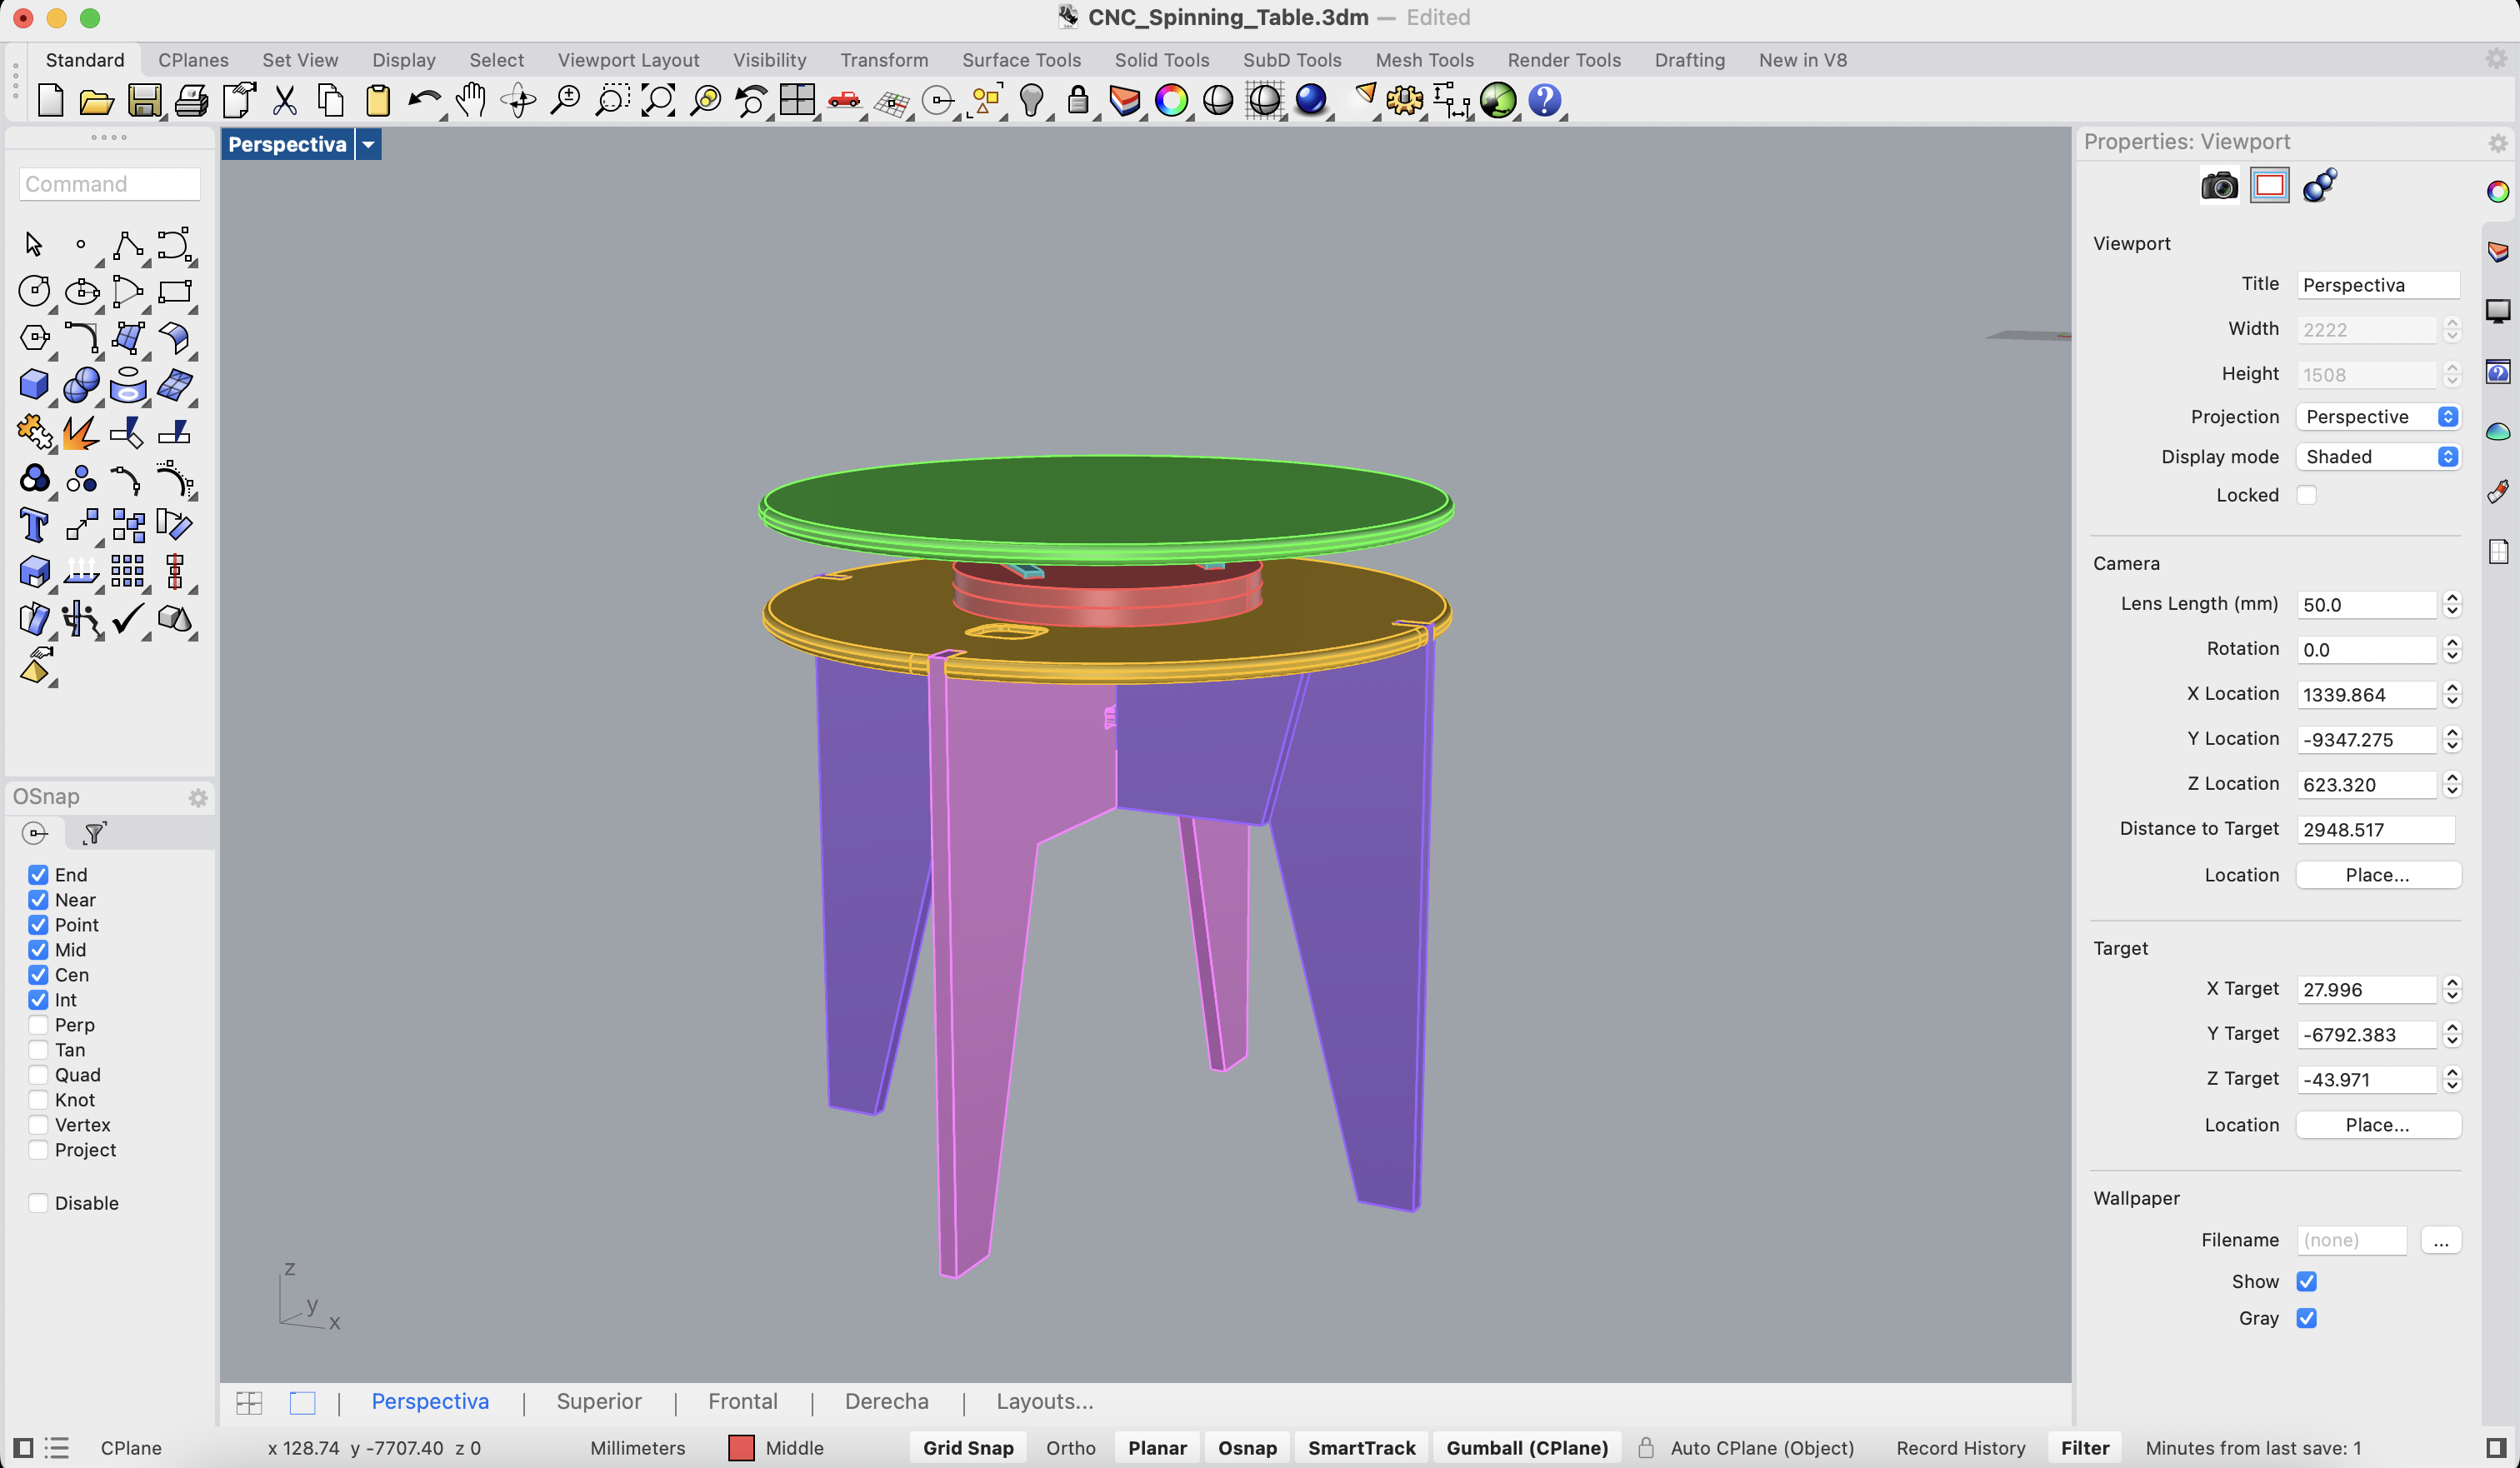
\includegraphics[width=1\textwidth]{figures/chapter3/RHINO_1.png}
\caption{Rhinoceros Interface. Source: Author}
\label{fig:rhino_interface}
\end{figure}

\subsection{\textit{AI Tools}: Natural Language as Input Mechanism}

The \textit{AI Tools} plugin creation looked to understand how natural language could work as an input mechanism for generating 3D content within existing Grasshopper workflows. The text-to-CAD component enabled makers to describe desired objects in everyday language, receiving geometrically precise 3D models suitable for fabrication. Prompts\footnote{In the context of AI and machine learning, a prompt is a specific input or instruction given to an AI system to guide its output.} like \textit{"Design a LEGO module with four connectors"} or \textit{"Create a bracket for mounting a sensor"} generated specific geometries that could be immediately integrated into larger parametric designs\footnote{Parametric designs are digital models created using parameters and relationships between geometric elements. Rather than fixed geometries, parametric models respond to input changes, allowing designers to explore variations by modifying underlying parameters while maintaining design logic and constraints.}.

\begin{figure}[H]
\centering
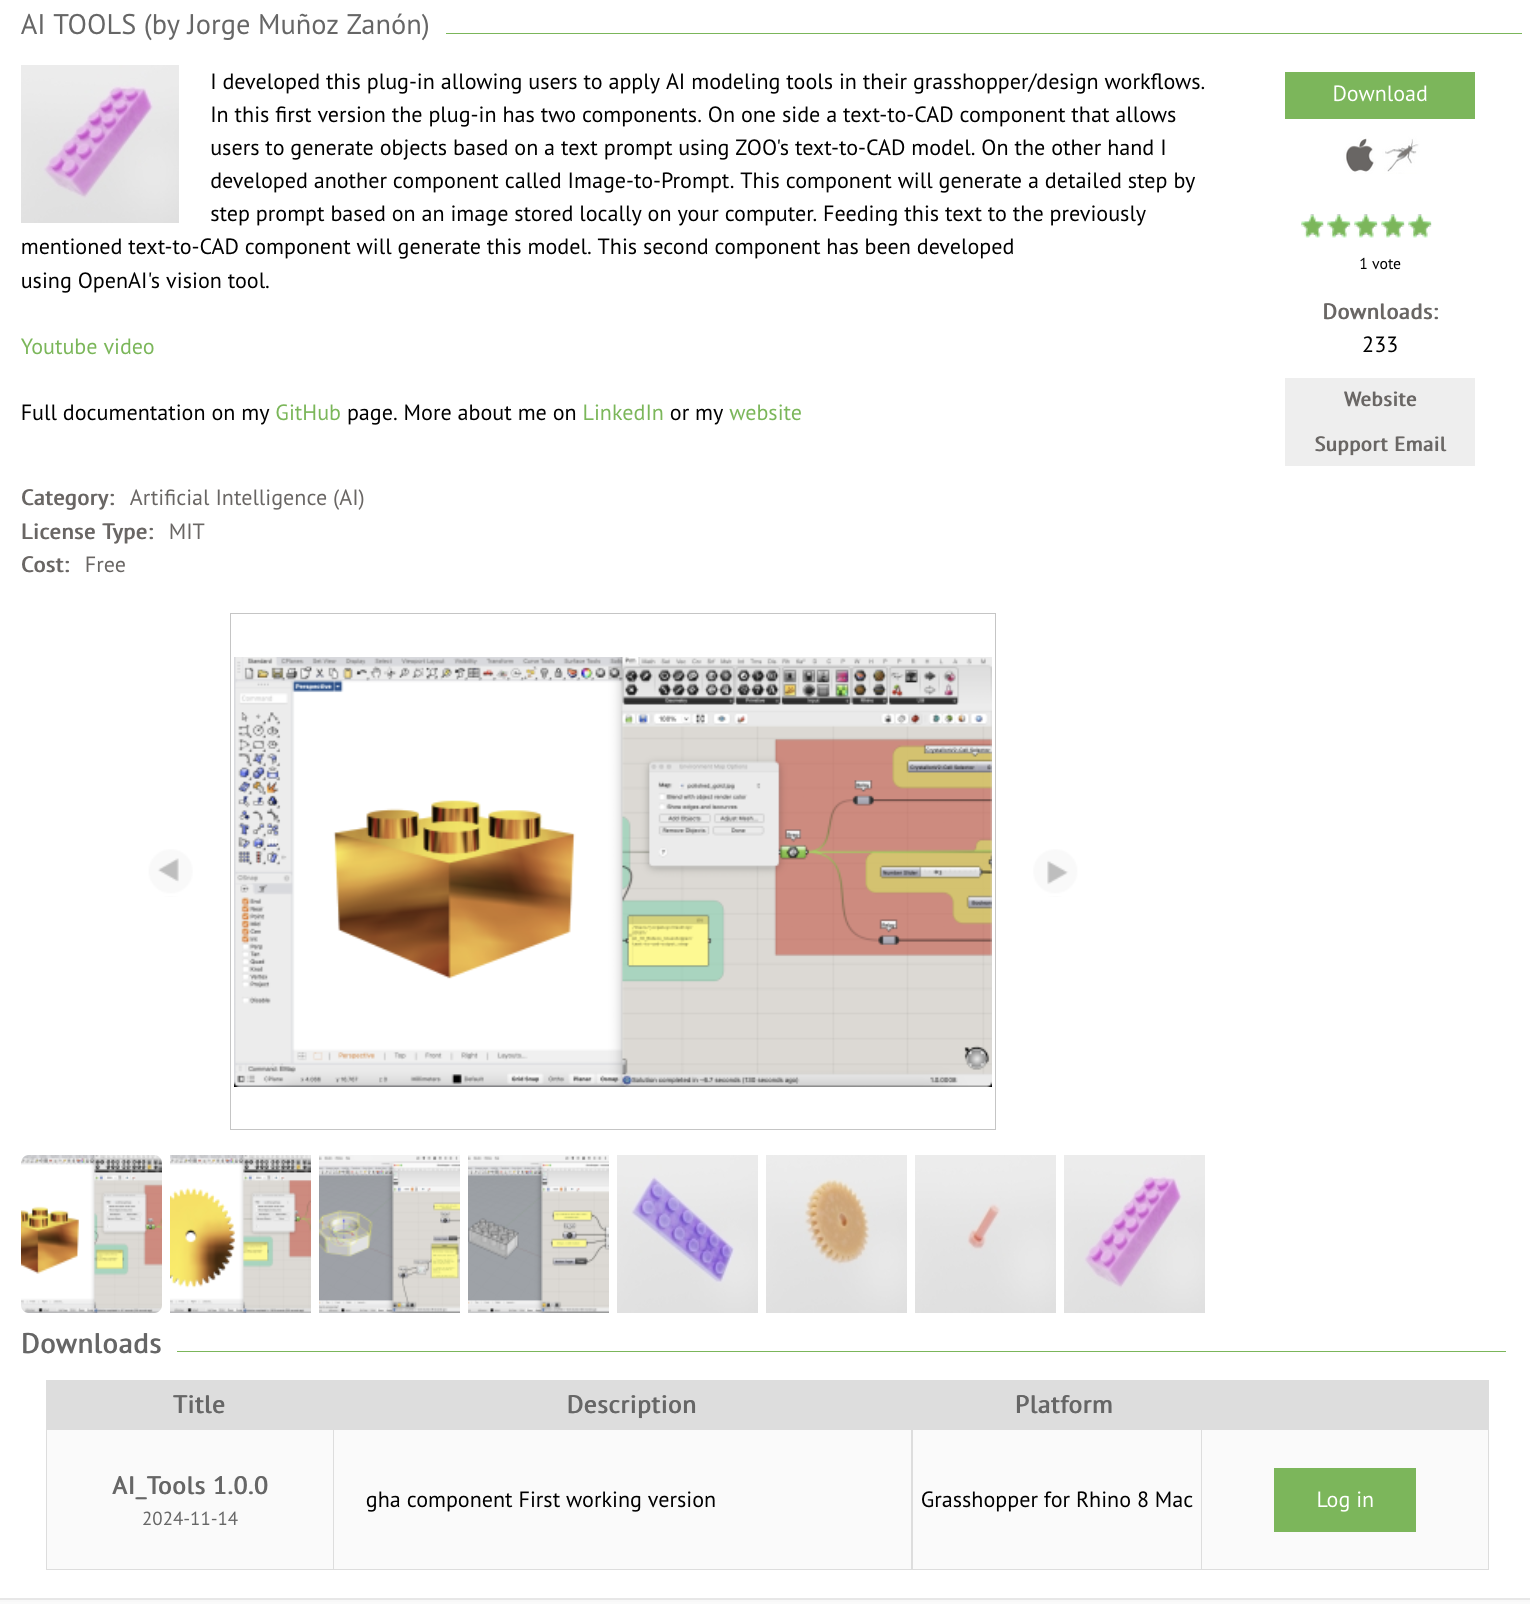
\includegraphics[width=1\textwidth]{figures/chapter3/AI_Tools.png}
\caption{Food4Rhino AI Tools Plug-In. Source: Author}
\label{fig:ai_tools}
\end{figure}

Through this approach, it was possible to identify several advantages over traditional geometric modeling. First, it enabled rapid exploration of form concepts without requiring detailed knowledge of 3D modeling techniques. Makers could iterate through multiple design variations by modifying textual descriptions rather than reconstructing geometric relationships. Second, it provided access to complex geometries that might be difficult or time-consuming to model manually.

\begin{figure}[H]
\centering
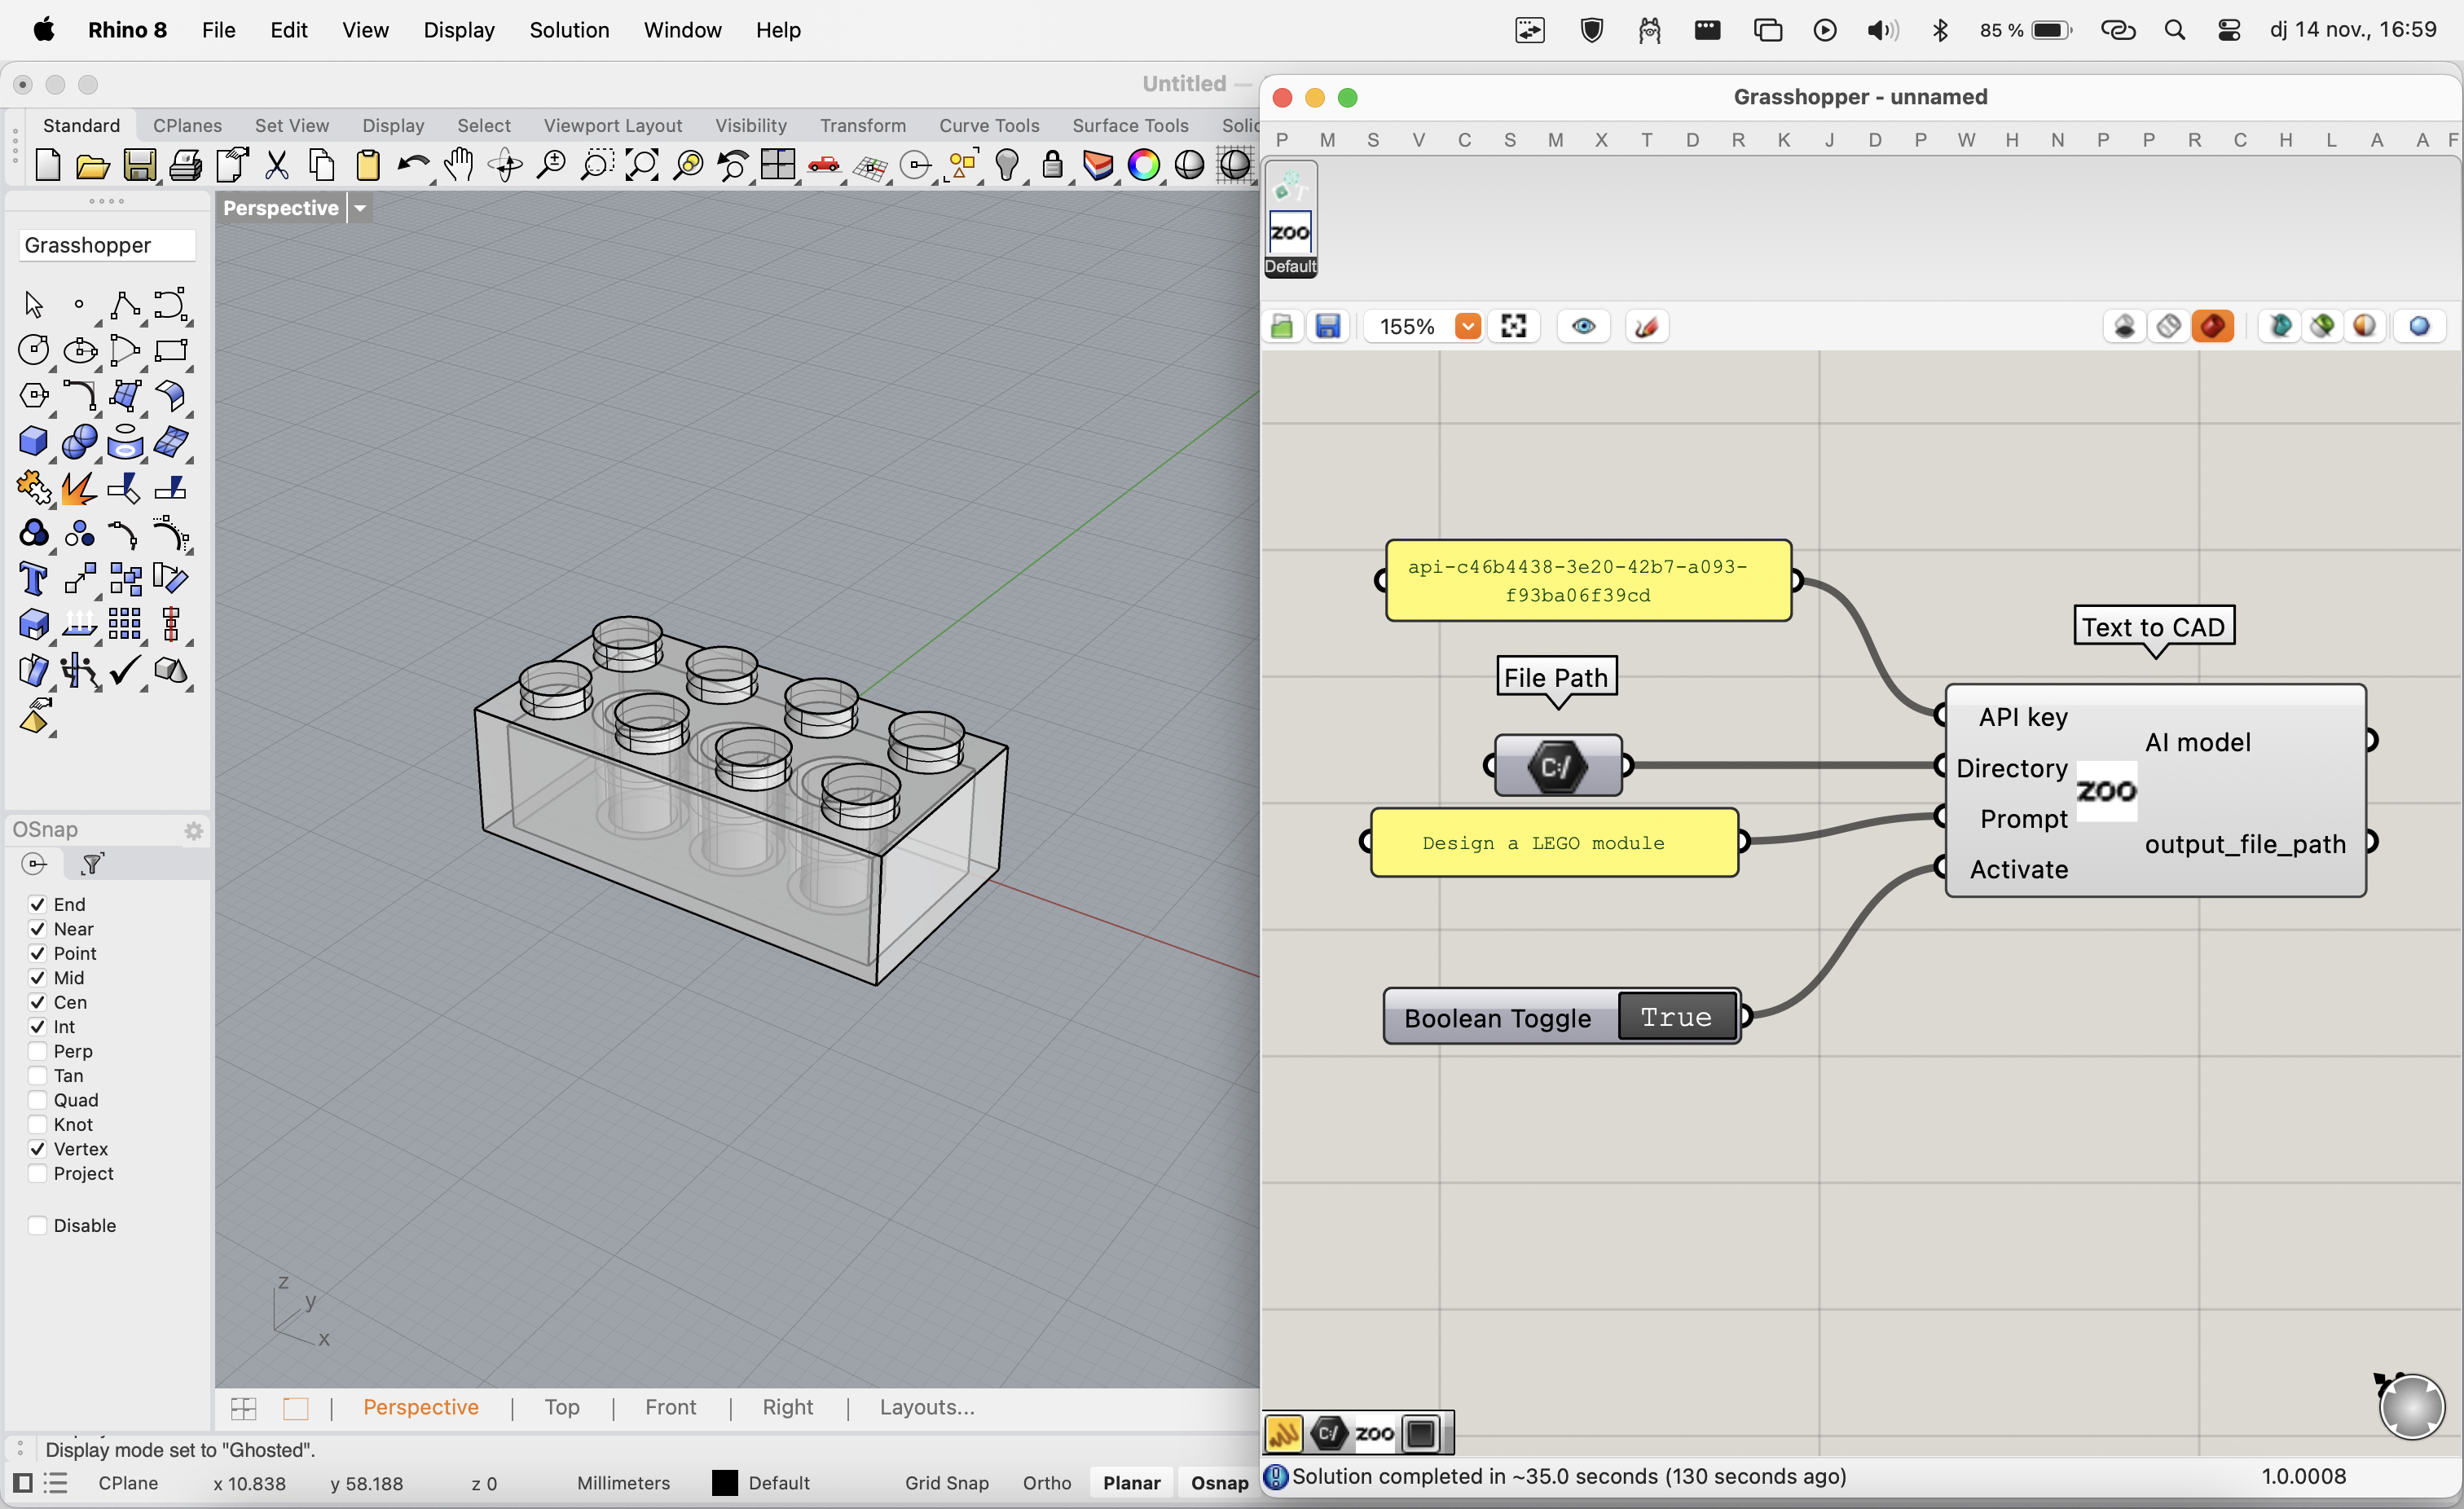
\includegraphics[width=1\textwidth]{figures/chapter3/text-to-cad.png}
\caption{Text-to-CAD Component. Source: Author}
\label{fig:text-to-cad}
\end{figure}

The image-to-prompt component extended this linguistic approach by enabling visual references to be translated into textual descriptions. Users could upload photographs, sketches, or existing objects to generate detailed natural language descriptions suitable for feeding into the text-to-CAD workflow. This created a multimodal conversation where visual, textual, and geometric representations could be fluidly translated between each other.

\begin{figure}[H]
\centering
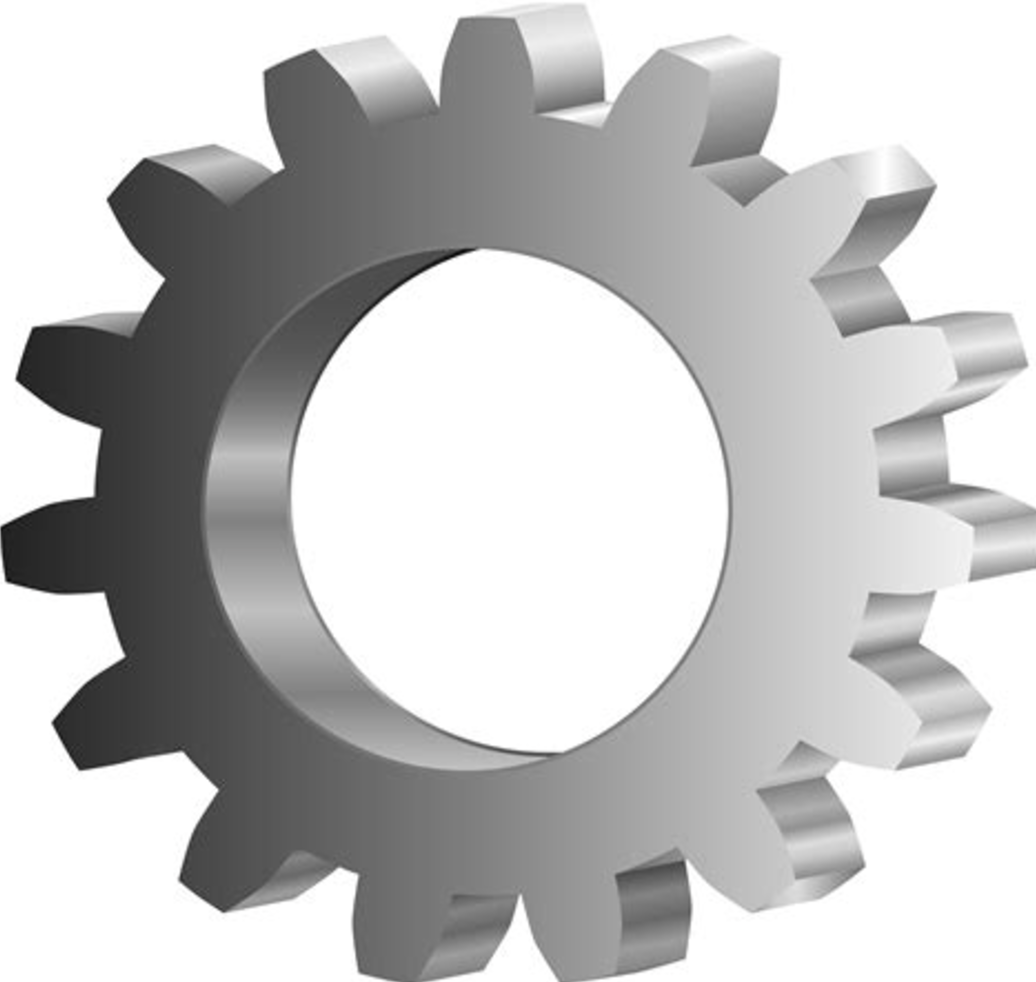
\includegraphics[height=5cm]{figures/chapter3/image-to-prompt-1.png}
\hspace{1cm}
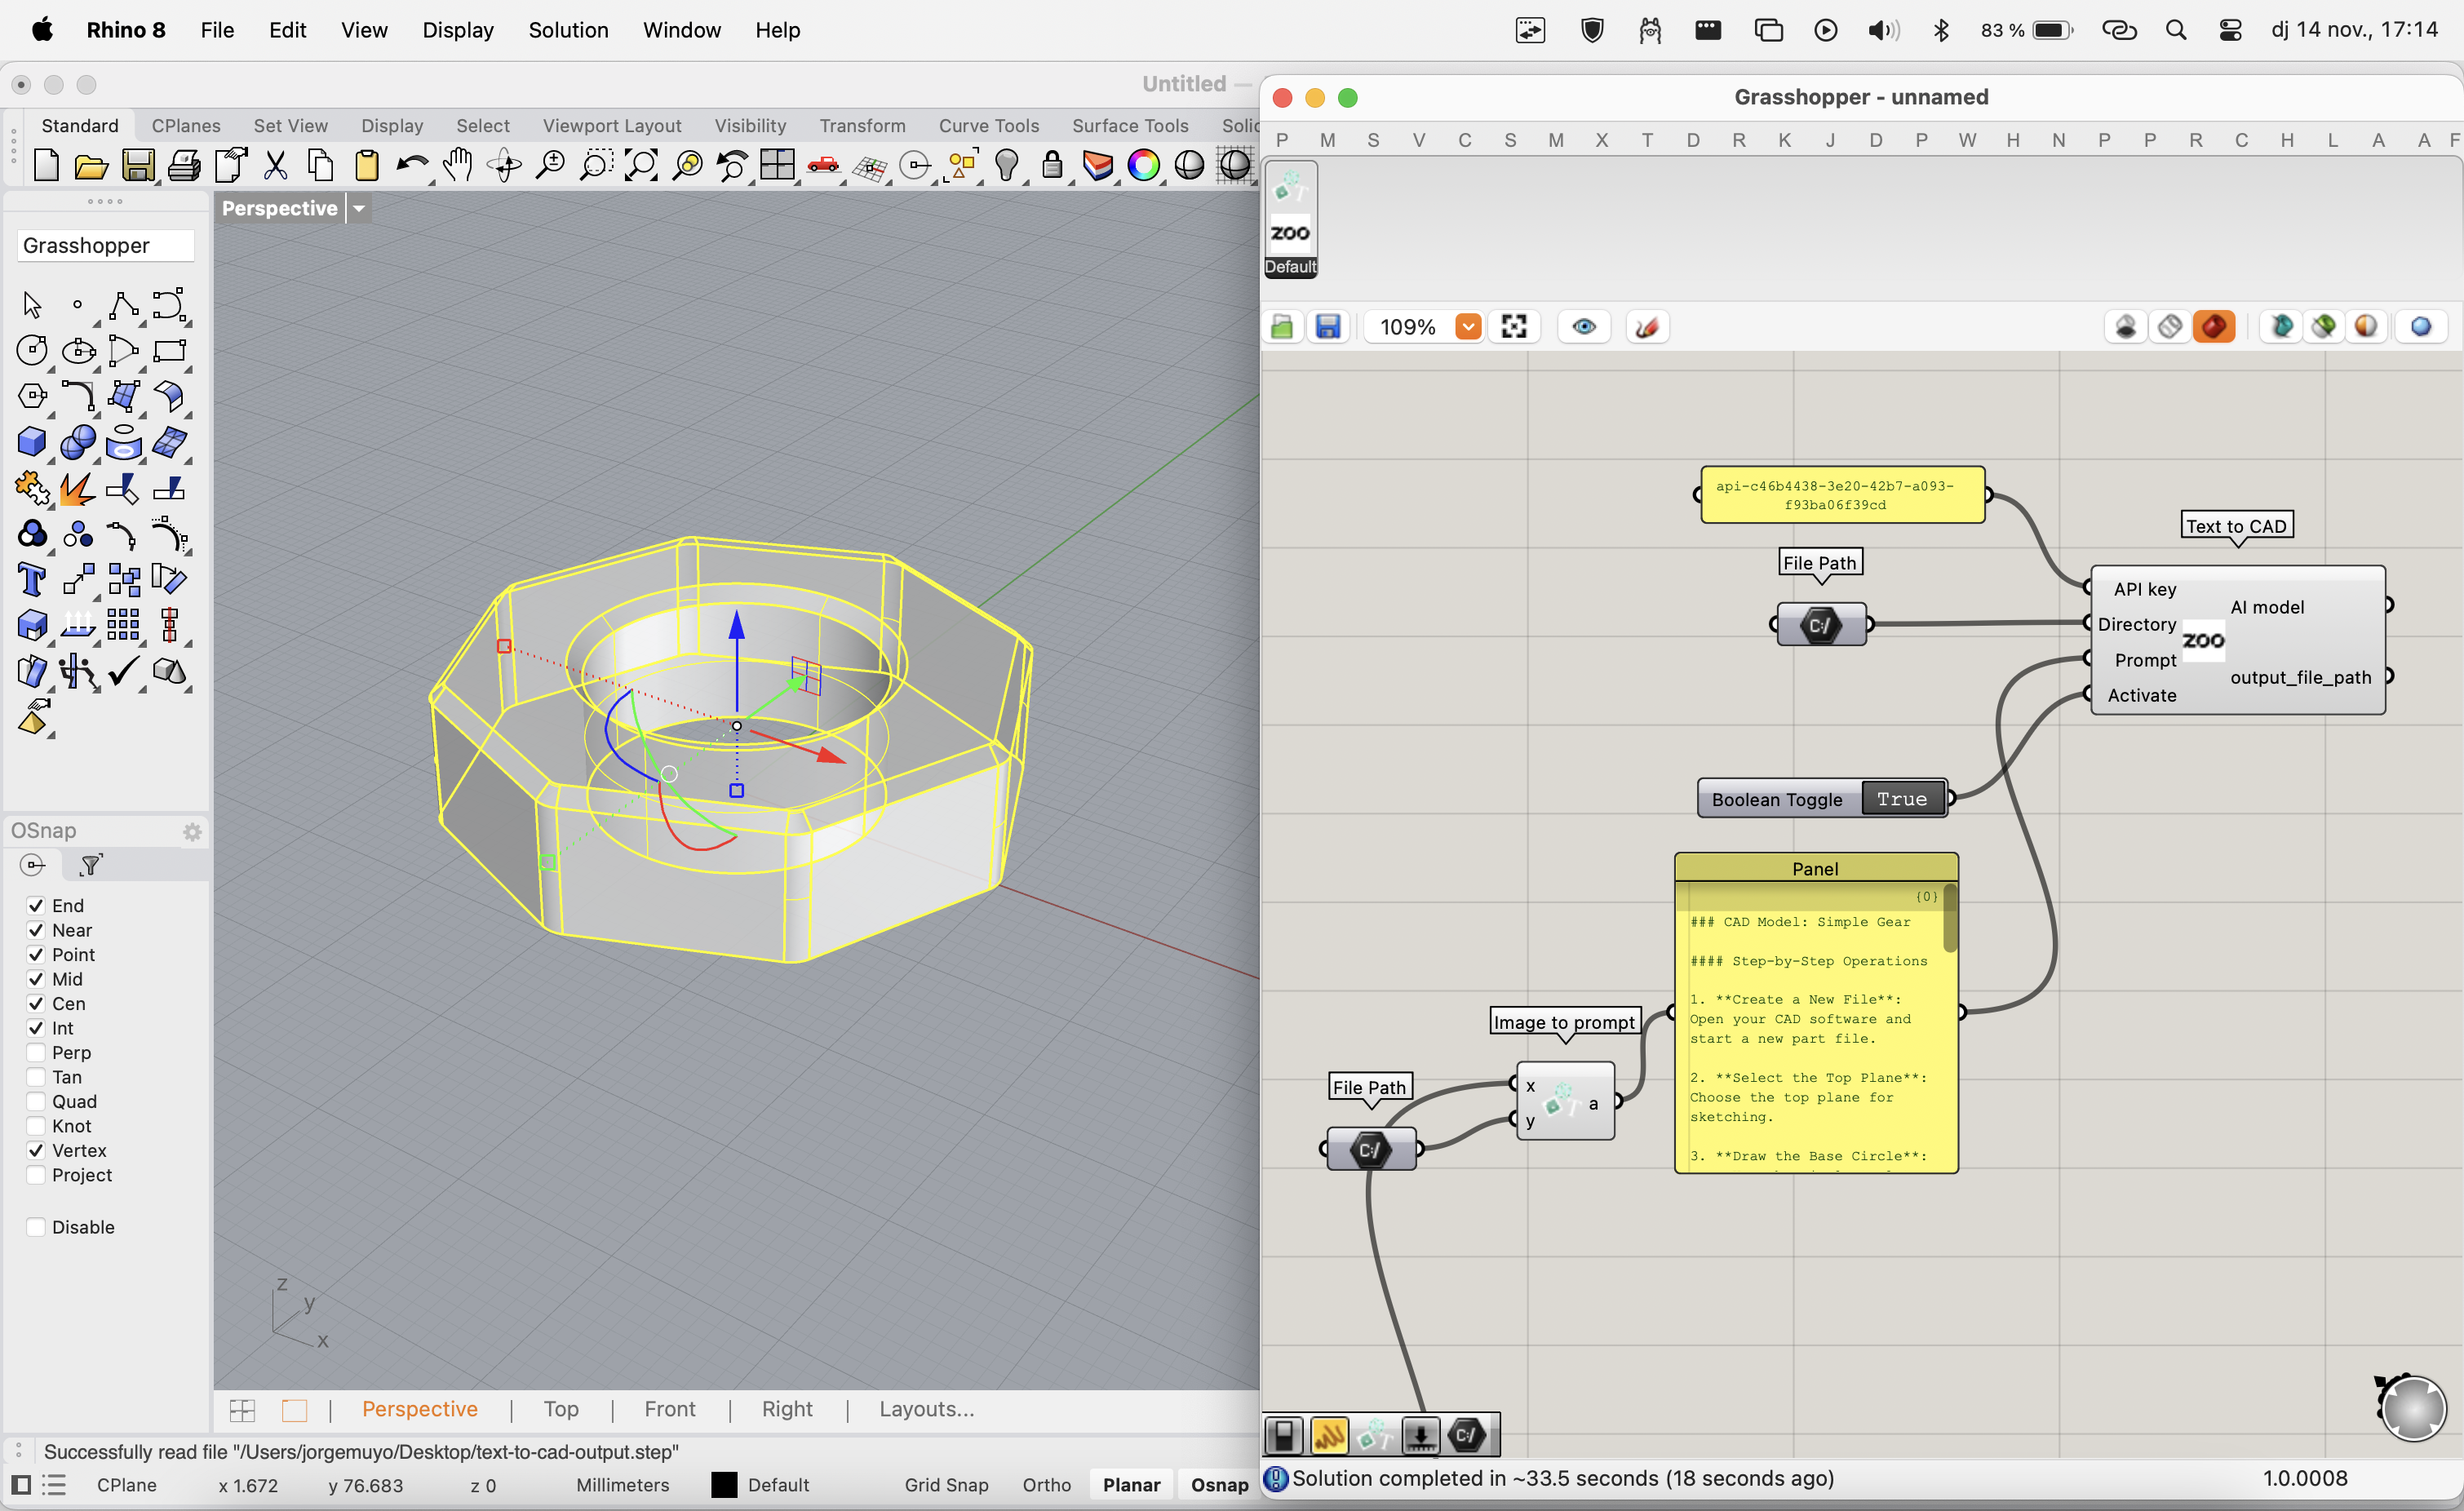
\includegraphics[height=5cm]{figures/chapter3/image-to-prompt-2.png}
\caption{Image-to-Prompt component. Sources: \citet{yopriceville_gear}, Author}
\label{fig:image-to-prompt}
\end{figure}

However, the through the use of \textit{AI Tools} certain limitations surfaced around treating language as simply another input mechanism. While natural language enables more intuitive specification of design intentions, the AI system's interpretation of those intentions operates through opaque training processes whose biases and assumptions remain unknown to makers. More importantly, the delivery of fully formed 3D models as outputs eliminates the very obstacles, negotiations, and material resistances that constitute the essence of making experience. By providing immediate geometric solutions, the system bypasses the iterative problem-solving, material dialogue, and adaptive decision-making that enable makers to develop embodied knowledge and maintain creative agency throughout the making process. This creates a form of creative "short circuiting" where technological efficiency undermines the experiential foundations of skilled practice, replacing the continuous negotiation between intention and material reality with predetermined computational outcomes.

\subsection{The \textit{Component That Makes}: Conversational Tool Building}

On the other hand, the \textit{Component that Makes} represents a more speculative exploration of language-mediated interaction, investigating how natural language could be used not just to generate predetermined content but to modify the computational environment itself. Rather than providing predetermined functionality, the component enables makers to describe needed capabilities and receive custom-generated Grasshopper components that become additions to their creative toolkit.

\vspace{0.5cm}

This approach transforms language from just an input mechanism into a tool for collaborative tool building. Makers can request components like \textit{"Create a tool that distributes objects along a curve with random rotation"} or \textit{"Generate a component that analyzes a mesh topology and identifies polygon concentration points"} The AI system will generate, compile, and install custom \textit{C\#}\footnote{\textit{C\#} (pronounced "C-sharp") is a general-purpose programming language developed by Microsoft. Within Grasshopper, C\# scripting components allow users to write custom algorithms and extend the software's functionality beyond its built-in components.} components that provide exactly the specified functionality, enabling makers to expand their computational vocabulary through conversation.

\vspace{0.5cm}

The \textit{Component that Makes} showcased several points of interest. First, it preserved transparency by providing complete generated source code (with comments) alongside functional components, enabling makers to understand and modify the AI-generated solutions. Second, it enabled iterative refinement through follow-up requests that built upon previous components, creating conversational workflows where computational tools emerged through dialogue.

\vspace{0.5cm}

The component generator's most intriguing characteristic exists in how it treated the Grasshopper canvas as collaborative documentation. Each generated component preserved not just a computational solution but a record of the conversational process through which that solution emerged. The component's parameters, connections, and modifications documented an ongoing dialogue between human intentions and AI interpretation, creating a conversational artifact that embedded linguistic interaction within the workflows.

\subsection{Toward Integrated Human-Software-Machine Dialogue}

The AI explorations showcased a big distinction between AI applications that automate creative processes versus those that expand creative capabilities. While text-to-CAD components delivered impressive technical results, they ultimately diminished maker agency by providing predetermined solutions that eliminated the iterative negotiation essential to skilled practice. The \textit{Component that Makes} approach, by contrast, worked as a transparent tool-building mediator that expanded rather than replaced human creative capabilities.

\vspace{0.5cm}

Beyond their differences, these experiments helped understand that conversational interfaces could bypass the need for simplification that had limited previous interface approaches. Rather than requiring makers to adapt their thinking to predetermined software logic, language-mediated interaction enabled creative intention to be expressed in natural human terms while maintaining computational sophistication, representing a reversal of the usual adaptation dynamic, instead of humans conforming to machine logic, the system adapted to human expression patterns.

\vspace{0.5cm}

The persistent documentation capabilities of conversational workflows offered another important insight. Unlike traditional CAD history that records geometric operations, conversational artifacts preserved the reasoning behind creative decisions, creating workflows that could be understood, modified, and built upon by future collaborators, suggesting pathways toward design and fabrication systems that maintained creative narratives alongside technical specifications.

\vspace{0.5cm}

However, the explorations also revealed limitations in language-based approaches. Natural language's ambiguity, its constraints in capturing embodied knowledge, and AI systems' dependence on existing training data and patterns indicate that linguistic interaction alone cannot fully address the preservation challenges defined inthis research. 

\section{Synthesizing Insights for Unified Agency}

The experimental progression from \textit{CR3ATED} through \textit{AI Tools} to the \textit{Component that Makes} highlighted a trajectory towards the goal of preserving creative agency within digital workflows, with each intervention contributing with different insights: \textit{CR3ATED} made clear the importance of maintaining material relationships through interface design, \textit{AI Tools} showcased the potential and limitations of automated content generation, and the \textit{Component that Makes} how different ways of interaction could expand human creative capabilities.

\vspace{0.5cm}

These findings converge on a clear goal: effective preservation-based democratization cannot be achieved through individual tools or techniques alone. Instead, it requires integrated systems that combine multiple ways of creative expression within unified workflows.

\vspace{0.5cm}

This synthesis of insights informed the development of \textit{Ars Post Faber}, an approach that attempts to address the limitations identified while building upon their collective strengths.